
\documentclass[a4paper,10pt,fleqn, twocolumn]{IEEETran}
\usepackage{amsfonts}
\usepackage{amsthm}
\usepackage{graphicx}
\usepackage{fancyhdr}

\newtheorem{Prop}{Proposition}
\newtheorem{lemma}{Lemma}


\setlength{\parindent}{3em} \setlength{\oddsidemargin}{0in}
\setlength{\textwidth}{6.5in} % sets 1in left and right margins
\setlength{\topmargin}{0.20in} % change to 0.2in for regular latex
%\setlength{\headheight}{0in}
%\setlength{\footheight}{0.5in}
\setlength{\footskip}{0.5in}
\setlength{\textheight}{9.0in} %sets 1in top and bottom margins
\renewcommand{\baselinestretch}{1} %set to 1.5 for double spacing.



\newcommand{\br}{{\mathbf r}}
\newcommand{\bA}{{\mathbf A}}
\newcommand{\ba}{{\bf a}}
\newcommand{\bb}{{\bf b}}
\newcommand{\bc}{{\bf c}}
\newcommand{\bC}{{\bf C}}
\newcommand{\bg}{{\bf g}}
\newcommand{\bG}{{\bf G}}
\newcommand{\bd}{{\bf d}}
\newcommand{\be}{{\bf e}}
\newcommand{\bq}{{\bf q}}
\newcommand{\bs}{{\bf s}}
\newcommand{\bm}{{\bf m}}
\newcommand{\bn}{{\bf n}}
\newcommand{\bu}{{\bf u}}
\newcommand{\bv}{{\bf v}}
\newcommand{\bw}{{\bf w}}
\newcommand{\bx}{{\bf x}}
\newcommand{\by}{{\bf y}}
\newcommand{\bbf}{{\bf f}}
\newcommand{\bE}{{\bf E}}
\newcommand{\bF}{{\bf F}}
\newcommand{\bL}{{\bf L}}
\newcommand{\bM}{{\bf M}}
\newcommand{\bN}{{\bf N}}
\newcommand{\bS}{{\bf S}}
\newcommand{\bT}{{\bf T}}
\newcommand{\bD}{{\bf D}}
\newcommand{\bX}{{\bf X}}
\newcommand{\bP}{{\bf P}}
\newcommand{\bQ}{{\bf Q}}
\newcommand{\bI}{{\bf I}}
\newcommand{\bR}{{\bf R}}
\newcommand{\bU}{{\bf U}}
\newcommand{\bV}{{\bf V}}
\newcommand{\bW}{{\bf W}}
\newcommand{\bJ}{{\bf J}}
\newcommand{\bB}{{\bf B}}
\newcommand{\bzero}{{\bf 0}}
\newcommand{\bgamma}{{\mbox {\boldmath $\gamma$}}}
\newcommand{\btheta}{{\mbox {\boldmath $\theta$}}}
\newcommand{\bLambda}{{\mbox {\boldmath $\Lambda$}}}
\newcommand{\bPsi}{{\mbox {\boldmath $\Psi$}}}
\newcommand{\bPhi}{{\mbox {\boldmath $\Phi$}}}
\newcommand{\bcA}{{\mbox {\boldmath ${\cal A}$}}}
\newcommand{\bcB}{{\mbox {\boldmath ${\cal B}$}}}
\newcommand{\bcC}{{\mbox {\boldmath ${\cal C}$}}}
\newcommand{\bcD}{{\mbox {\boldmath ${\cal D}$}}}
\newcommand{\bcF}{{\mbox {\boldmath ${\cal F}$}}}
\newcommand{\bcN}{{\mbox {\boldmath ${\cal N}$}}}
\newcommand{\bcR}{{\mbox {\boldmath ${\cal R}$}}}
\newcommand{\bcS}{{\mbox {\boldmath ${\cal S}$}}}
\newcommand{\bcH}{{\mbox {\boldmath ${\cal H}$}}}
\newcommand{\bcI}{{\mbox {\boldmath ${\cal I}$}}}


\title{Blind Interference Cancellation}
\author{Shu Wang, Sang G. Kim, Li-Hsiang Sun, Hobin Kim,\\
   Suk W. Lee, S. R. Subramanya, Ki Y. Kim and Byung K. Yi\\ LGE Mobile Research (LGEMR), San Diego, CA 92131}
\date{}
\begin{document}
\maketitle
\begin{abstract}\small
Compensating for near-far effects is critical for satisfactory
performance of code division multiple access (CDMA) systems.
Interference cancellation is one of the multiuser detection (MUD)
strategies for suppressing multiple access interference (MAI)
effects and consequently improving the system performance. In this
paper, several blind interference cancellers based on least-square
(LS), minimum mean-square error (MMSE) criteria and blind
multiuser model are proposed for solving solving the near-far
problem in synchronous CDMA. Compared with existing blind
multiuser detectors, the proposed detectors require a minimum
number of previously received signals and no subspace separation
or channel/sequence estimation operation. And their computation
complexity can be much lower and detection delays are much
reduced. All these can be easily extended for asynchronous CDMA.
Theoretical analysis and computer simulations are provided to
demonstrate the performance of the proposed schemes.
\end{abstract}
\section{Introduction}
Multiuser detection strategy is a method for mitigating multiple
access interference (MAI) effects and solving the near-far problem
with exploiting interference structure~\cite{Verd98}. Recent
research has been devoted to blind multiuser detection and
subspace-based signature waveform estimation schemes for achieving
better performance and higher
capacity~\cite{Madh94,Honi95,Torl97,Wang98,Wang99,Zhang02}. Blind
multiuser detectors can achieve good performance with only the
knowledge of the timing and signature waveform of desired user(s).
This assumption also is much closer to practical applications.
There are two popular approaches for designing blind multiuser
detectors. One is to use the conventional multiuser signal
model~\cite{Verd98,Madh94,Honi95,Zhang02} and the other approach
is based on parametric signal modelling and signal spectrum
estimation~\cite{Wang98,Wang99}.

Interference
cancellation~\cite{Yoon93,Patel94,Wijk95,Divsalar96,Kim98,Bugallo01}
provides a promising alternative to the conventional or optimum
detectors in multiuser detection since they typically require less
implementation complexity while practically offering similar
performance. The idea behind IC is to form an estimate of the
multiple access and/or multipath induced interference and then
subtract the interference estimate from the received signal.
Hence, compared to most MUD schemes, IC pays more attention to the
estimation of the MAI. Different schemes for the MAI estimation
lead to different IC schemes. Actually, an IC detector will cancel
the interfering signal exactly provided that the decision was
correct and channel information is known. Otherwise, it may
increase the contribution of the interferers. The main
alternatives for implementation of IC are parallel hard
interference cancellation (PIC)~\cite{Divsalar96,Kim98} and
serial/successive hard interference cancellation
(SIC)~\cite{Patel94,Wijk95}, while many other variants on these
basic principles have also been developed. With conventional PIC,
all users are simultaneously demodulated and detected in a
parallel fashion. With conventional SIC, the users are ordered,
usually by decreasing received power, and demodulated
successively. The prior users contribution to the received signal
is removed for each successive user such that each successive user
sees less and less interference.

One of the major difficulties in designing blind multiuser
detector or interference cancellor is receivers have no enough
spreading signature information for received signals, which make
it difficult to estimate the desired users' bits directly. One of
the typical approaches for solving this problem is to do blind
sequence or receiver filter estimation using statistical signal
processing techniques including subspace-based techniques. Here we
take an alternative non-statistical approach for interference
cancellation. We firstly introduced a so-called blind spreading
matrix and represent received signal vectors in new fashion. We
then separate interference from received signals using
Gauss-Seidel transformation, estimate the MAI and do interference
cancellation.

In order to solve the near-far problem with minimum prior
knowledge and computation complexity, we propose several blind
interference cancellation schemes using a blind multiuser signal
model in this paper. This blind signal model is different from the
traditional linear prediction model~\cite{Haykin96} and the
widely-discussed conventional signal model and subspace-based
parametric signal model. In the proposed model, each received
signal can be taken as a linear combination of desired users'
spreading sequences, several previously received signals and/or
noise. Based on this new blind multiuser signal model, several
blind interference cancellation schemes are developed using LS and
MMSE criteria for interference estimation. The proposed algorithms
are simple and direct only using the signatures and timing of
desired users. There is no converging, estimation or subspace
separation procedure employed by many other blind
detectors~\cite{Madh94,Honi95,Wang98,Wang99}. Compared with
existing blind detection schemes, they require a minimum number of
previously received signals. Hence the computation complexity and
detection delay can be much reduced. Theoretical analysis and
computer simulations are finally presented to demonstrate the
performance of these blind detectors.
\section{System Model And Problem Description}
We consider forward-link transmissions in a single-cell DS/CDMA
system. There are $K$ active users over the multipath channel with
$P$ strong paths~\footnote{Strong paths are those to be explicitly
combined by RAKE receiver.} and the channel is an additive white
Gaussian noise (AWGN) channel. The baseband representation of the
received signal due to user $k$ is given by
\begin{equation}
\begin{array}{rcl}
r_k(t)&=&\sum\limits_{p=1}^{P}\alpha_{pk}A_k[n]
b_k[n]c_k(t-nT-\tau_p)
\end{array}
\end{equation}
\noindent where $\alpha_{pk}$ is the $p$th path loss of user $k$'s
signal, $b_k{[n]}$ is the $n$th bit sent by user $k$. We assume
that the $\left\{b_k{[n]}\right\}$ are independent and identically
distributed random variables with $E\left\{b_k{[i]}\right\}=0$ and
$E\left\{|b_k{[i]}|^2\right\}=1$. The parameters $c_k(t)$ denote
the normalized spreading signal waveform of user $k$ during the
interval $[0,\ T]$, $\tau_1\leq\tau_2\leq\ldots\leq\tau_P$,
denotes $P$ different transmission delays from the base station to
user $k$ and $A_k[n]$ is the amplitude of the received signal for
user $k$ at time $t=n$. The total baseband signal received by user
$k$ is
\begin{equation}
\begin{array}{rcl}
\tilde{r}(t)&=&\sum\limits_{k=1}^{K}r_k(t)
\end{array}
\end{equation}
The received signal $\tilde{r}(t)$ is passed through the
corresponding chip matched filter (CMF) $\phi(t)$ and RAKE
combiner. The combined output $r(t)$ is~\footnote{Without loss of
the generality, we drop the time index $n$ in the following
discussion.}
\begin{equation}\hspace{-0.0in}
\begin{array}{rcl}
r(t)&=&A_k b_k c_k(t-nT-\tau_1)\otimes \phi(t-\tau_1)+ \\
&&\hspace{0.0in} m_{\rm ISI}(t) + m_{\rm MAI}(t) + n(t)
\end{array}\label{r_t}
\end{equation}
\noindent where
\begin{equation} \hspace{-0.05in}
\begin{array}{rcl}
 m_{\rm ISI}(t)&=&\\
 &&\hspace{-0.83in}\sum\limits^{P}_{p\neq
q}\beta_{qk} \alpha_{pk}A_kb_kc_k(t-nT+\tau_{q1}-\tau_1)\otimes
\phi(t-\tau_1)
\end{array}
\end{equation}
\noindent is the intersymbol interference (ISI) to user $k$,
\begin{equation} \hspace{-0.17in}
\begin{array}{rcl}
m_{\rm MAI}(t)&=&\sum\limits_{i\neq
 k}^{K}A_ib_ic_i(t-nT-\tau_1)\otimes\phi(t-\tau_1)+\\
 &&\hspace{-0.75in}\sum\limits_{i\neq
 k}^{K}\sum\limits^{P}_{p\neq
q}\beta_{qk}
\alpha_{pi}A_ib_ic_i(t-nT+\tau_{q1}-\tau_p)\otimes\phi(t-\tau_1)
\end{array}
\end{equation}
\noindent is the MAI to user $k$, $\beta_{qk}$ is the weight of
the $q$th RAKE finger with
$\sum\limits_{q=1}^{P}\beta_{qk}\alpha_{qk}=1$ and $\tau_{q1} =
\tau_{q}-\tau_1$ is the propagation delay difference between the
$1$st path and $p$th path. $\otimes$ denotes the convolutional
product. $n(t)$ is AWGN with variance $\sigma^2$. The user $k$'s
RAKE output can be sampled at $f_s=1/T_s$ and straightforwardly
expressed by
\begin{equation}\hspace{-0.1in}
\begin{array}{rcl}
\br&=&\left[
\matrix{r(nT+T_s+\tau_1)&\ldots&r(nT+LT_s+\tau_1)}\right]^{\rm
T}\\
 &=&\sum\limits_{k=1}^{K} A_k b_k \bs_k + \bn \\
 &=&\bS \bA \bb + \bn
\end{array}\label{r_sync}
\end{equation}
\noindent where $\bS=[\bs_1\ \bs_2\ \ldots\ \bs_K]$ is the
received spreading sequence matrix combined with both ISI and MAI
information, and $L=T/T_s$ is the number of samples per symbol,
which should not be less than the spreading gain $L_c$.

Because of $m_{\rm MAI}(t)$ existing in the received signal
$r(t)$, the performance of conventional matched filter receiver
suffers from the so-called near-far problem~\cite{Verd98}.
Multiuser detection is the receiver technique for solving this
problem and most multiuser detectors are firstly developed using
the conventional system model like (\ref{r_sync}). These are well
documented in~\cite{Verd98}. One of the difficulties in developing
blind multiuser detectors using (\ref{r_sync}) is that the $\bS$
is hard to be known beforehand. And it normally takes much effort
to determine it later. The similar situation can also be met in
developing blind detectors using the parametric subspace signal
model proposed in~\cite{Wang98}.

\section{Blind Interference Cancellation}

In order to blindly estimate MAI without the original spreading
matrix $\bS$, we use a new blind but "faked" spreading matrix
$\bcS$ instead. We call it the blind but "faked" spreading matrix
because 1) it is composed by only desired users' spreading
sequences and previously received signals and 2) it isn't the
original one but will work like the original one. Without loss of
the generality, only the bits sent for first $G$ users are
considered here and the $L\times M$ blind spreading sequence
matrix $\bcS$ is defined by
\begin{equation}
\begin{array}{rcl}
\bcS&=&\left[\matrix{\bcS_1&\bcS_2}\right]\\
&=&\left[\matrix{\bs_1&\ldots&\bs_G&{\br}_{1}&{\br}_{2}&\ldots&{\br}_{M-G}}\right]
\end{array} \label{S_0}
\end{equation}
\noindent where
$\bcS_1=\left[\matrix{\bs_1&\bs_2&\ldots&\bs_G}\right]$ and
$\bs_g$, $g=1,\ 2,\ \ldots,\ G$, denote the group of $G$ known
spreading waveforms to user $1$.
$\bcS_2=\left[\matrix{\br_1&\br_2&\ldots&\br_{M-G}}\right]$ and
${\br}_m$, $m=1,\ 2,\ \ldots,\ M-G$, are $M-G$ previously received
independent signal vectors~\footnote{The first $M-G$ received
signal $\br_m$ may be obtained from some receiver initialization
procedure. After that, there will be some possible adaptive
procedure for updating $\bcS$, e.g. the procedure proposed in
Section \ref{updatingG}. Compared with existing blind detectors,
this number, $M-G$, of required previously received signals are
very small.}. $K\leq M\leq L$. Obviously $M=K$ is the minimum
number for blind multiuser detector to unambiguously distinguish
different interfering signals. And if $M>L$, blind multiuser
receiver will not be unique since there will be more variables
than available equations. The relationship between the proposed
blind spreading matrix $\bcS$ and the original spreading matrix
$\bS$ can be given by
\begin{equation}
\begin{array}{rcl}
\bcS &=&\bS\bB + {\bN}\\
\end{array}\label{S_1}
\end{equation}
\noindent where the first $G$ columns of $\bcS$ and $\bS$ are
same,
\begin{equation}\hspace{-0.0in}
\begin{array}{c}
 \bB=\left[\matrix{\bI & \bar\bD\cr\bzero&\tilde\bD }\right]=\left[\matrix{\bE & \matrix{\bar\bD\cr \tilde{\bD}} }\right]
  =\left[\matrix{\bG \cr \matrix{\mathbf{0}& \tilde{\bD}}
 }\right]
\end{array}\label{B}
\end{equation}
\noindent is the $K\times M$ data matrix associated with $\bcS$.
$\bE=[\matrix{\bI&\bzero}]^{\rm T}$, $\bG = \left[\matrix{\bI&
\bar\bD}\right]$ is the $G\times M$ matrix composed by known data
in $\bcS$. $\mbox{rank}\{\tilde{\bD}\}=K-G$ and
$\mbox{rank}\{\bB\}\leq K$.

After the blind spreading matrix $\bcS$ is defined, the received
signal vector $\br$ in (\ref{r_sync}) can be expressed as the
linear combination of the columns in $\bcS$ instead of $\bS$ by
\begin{equation}
\begin{array}{rcl}
\br&=&\bcS\bbf + \bar{\bn}\label{r_blind}
\end{array}
\end{equation}
\noindent where the $M \times 1$ vector $\bbf$ is termed the
detection vector defined by
\begin{equation}
\begin{array}{rcl}
\bbf&=&\left[\matrix{\bbf_1^{\rm H}&\bbf_2^{\rm H}}\right]^{\rm H} \\
&=&\bB^{+}\bar\bb
\end{array} \label{DetectorVector}
\end{equation}
\noindent where $\bbf_1$ is the subvector of $\bbf$ consisting of
the first $G$ elements of, $\bbf_2$ consists of the rest $M-G$
elements, $[\cdot]^{+} $ denotes the general inverse operator and
$\bar\bb=\bA \bb$. $\bar{\bn}$ is the new $L\times 1$ noise vector
defined by
\begin{equation}
\begin{array}{rcl}
\bar{\bn}&=&\bn-{\bN}\bB^{+}\bar\bb
\end{array}. \label{new_noise}
\end{equation}
\noindent Meanwhile, the MAI part of $\br$ can be written by
\begin{equation}
\begin{array}{rcl}
\bm&=&\bS_2\bA_2\bb_2\\
&=&\left(\bcS_2-\bcS_1\bar\bD\right)\bbf_2
\end{array}\label{bm}
\end{equation}
\noindent where $\bS_2$, $\bA_2$ and $\bb_2$ denote the original
spreading sequences, amplitudes and information bits for
interfering users. In order to separate MAI from received signal
for estimating $\bbf_2$, we perform QR-decomposition on $\bS_1$ by
\begin{equation}
\begin{array}{rcl}
\bS_1&=&\bQ_1\bR_1
\end{array},
\end{equation}
\noindent where $\bQ_1\in\mathbb{R}^{L\times L}$ is orthogonal and
$\bR_1=[\bR_{11}^{\rm H}\ \bzero^{\rm H}]^{\rm
H}\in\mathbb{R}^{L\times G}$, and apply $\bQ_1^{\rm H}$ on both
sides of (\ref{r_sync}) and (\ref{r_blind}). We then get
\begin{equation}
\begin{array}{rcl}
\bQ_{1}^{\rm
H}\br&=&\left[\matrix{\bR_{11}\bA_1\bb_1\cr\bzero}\right]+\left[\matrix{\bR_{12}\bA_2\bb_2\cr\bR_{22}\bA_2\bb_2}\right]+\bQ_1^{\rm
H}\bn\\
&=&\left[\matrix{\bcR_{11}\bbf_1\cr\bzero}\right]+\left[\matrix{\bcR_{12}\bbf_2\cr\bcR_{22}\bbf_2}\right]+\bQ_1^{\rm
H}\bar\bn
\end{array}
\end{equation}
\noindent where the matrices $\bR_{11}$, $\bR_{12}$ and $\bR_{22}$
are given by
\begin{equation}
\begin{array}{rcl}
\bQ_{1}^{\rm
H}\bS&=&\left[\matrix{\bR_{11}&\bR_{12}\cr\bzero&\bR_{22}}\right]
\end{array}
\end{equation}

\noindent and the matrices $\bcR_{11}$, $\bcR_{12}$ and
$\bcR_{22}$ are given by

\begin{equation}
\begin{array}{rcl}
\bQ_{1}^{\rm
H}\bcS&=&\left[\matrix{\bcR_{11}&\bcR_{12}\cr\bzero&\bcR_{22}}\right]
\end{array}.
\end{equation}

 Now we can see that $\bbf_2$ can be estimated with solving

\begin{equation}
\begin{array}{rcl}
\left[\matrix{\bzero&\bI}\right]\bQ_{1}^{\rm
H}\br&=&\bcR_{22}\bbf_2+\left[\matrix{\bzero&\bI}\right]\bQ_1^{\rm
H}\bar\bn
\end{array}.
\end{equation}
\noindent After $\bbf_2$ is estimated, the MAI $\bm$ can be
estimation using (\ref{bm}) and finally the desired information
bits $\bb_1$ can be detected with solving

\begin{equation}
\begin{array}{rcl}
\br-\bm&=&\bS_1\bA_1\bb_1 + \bar{\bn}
\end{array}\label{br_bm}
\end{equation}

\subsection{Least-Square Interference Cancellation}



We can see that (\ref{r_blind}) may be taken as a modified linear
prediction model and the multiuser detection problem may be taken
a modified linear prediction problem~\footnote{Blind multiuser
detection using linear prediction will be discussed in another
paper.} if $\bar{\bn}=\bzero$. On the other hand, if $\bbf$ can be
estimated, the amplitudes $A_g$ and bits $b_g$ for the first $G$
users can be estimated and detected with (\ref{DetectorVector}) by
\begin{equation}\hspace{0.2in}
\begin{array}{l}
\hat{\bb}_1
=\left[\matrix{\hat{b}_1&\hat{b}_2&\ldots&\hat{b}_G}\right]^{\rm
T}=\mbox{sgn}\left\{\bG\bbf\right\}\
\end{array}, \label{b_estimation}
\end{equation}
\begin{equation}\hspace{-0.40in}
\begin{array}{l}
\hat{\ba}_1
=\left[\matrix{\hat{A}_1&\hat{A}_2&\ldots&\hat{A}_G}\right]^{\rm
T}=\left|\bG\bbf\right|\ .
\end{array} \label{A_estimation}
\end{equation}

In the following, we will present various schemes for estimating
$\bbf$ and detecting $\bb_1$. An adaptive implementation will be
presented in Section \ref{updatingG}.

\section{Blind Interference Cancellation}

Now we discuss the ideas using interference cancellation
techniques for estimating $\bbf$. At first, we note MAI as

\begin{equation}
\begin{array}{rcl}
\bm&=&\sum\limits_{k=G+k}^{K}A_kb_{k}\bs_k\\
&=&\bS_2\bA_2\bb_2\hspace{0.1in}.
\end{array}
\end{equation}

\noindent The received signal vector $\br$ can be written by

\begin{equation}
\begin{array}{rcl}
\br&=&\bcS\bbf+\bar\bn\\
&=&\bS_1\bA_1\bb_1+\bm+\bn\hspace{0.1in},
\end{array}
\end{equation}

\noindent where $\bS_1$ is the matrix composed by known $G$
signature vectors and its QR factorization is given by

\begin{equation}
\begin{array}{rcl}
\bS_1&=&\left[\matrix{\bs_1&\bs_2&\ldots\bs_G}\right]\\
 &=&\bQ_1\bR_1
\end{array}
\end{equation}

\noindent where $\bQ_1\in\mathbb{R}^{L\times L}$ is orthogonal and
$\bR_1\in\mathbb{R}^{L\times G}$. In order to estimate $\bm$ for
cancelling interference later, $\bQ_1^{\rm T}$ is applied to and
produce

\begin{equation}
\begin{array}{rcl}
\left[\matrix{\bR_1\bA_1\bb_1+\cr\bzero}\right]+\bQ_1^{\rm
T}\bm+\bQ_1^{\rm T}\bn&=&\bQ_1^{\rm T}\bcS\bbf+\bQ_1^{\rm
T}\bar\bn
\end{array}
\end{equation}









\noindent where $\bar\bs_m$ and $f_m$ are the $m$th column and
element of the blind spreading matrix $\bcS$ and the detection
vector $\bbf$, respectively. The interference cancellation idea
here for estimate





 In this section, another scheme
is proposed to estimate $\bm$ directly using $\bS$. It will be
shown that the estimated MAI, $\hat{\bm}$, for direct estimation
minimizes

\begin{equation}
\begin{array}{rcl}
\bm^{\rm
D-IC}&=&\mbox{arg}\min\limits_{\hat{\bm}}\left\|\hat{\bm}-(\br-b_1A_1\bs_1)\right\|_2\hspace{0.1in}.
\end{array}
\end{equation}

Before estimating $\bm$, a Householder transformation, $\bQ$, is
defined and applied to (\ref{r}) producing

\begin{equation}
\begin{array}{rcccl}
\bQ^T\br&=&\bar{\br}&=&\left[\matrix{r_1\cr\bar{\br}_2}\right]
\end{array}\label{Qr}
\end{equation}

\noindent and

\begin{equation}
\begin{array}{rcccl}
\bQ^T\bS&=&\bQ^T[\matrix{\bs_1&\tilde{\bS}}]&=&\left[\matrix{c&\bar{\bs}_{21}^T\cr\mathbf{0}&\tilde{\bS}_{22}}\right]
\end{array}\label{QS}
\end{equation}

\noindent where $r_1$ is the first element in the vector
$\bar{\br}$, $\bar{\br}_2$ is the $(L-1)\times 1$ complement
subvector of $r_1$, $\bar{\bs}_{21}$ is a $(K-1)\times 1$ vector
and $\tilde{\bS}_{22}$ is a $(L-1)\times (K-1)$ matrix and
$c=\pm\|\bs_1\|_2=\pm1$. This Household transformation can then be
written as

\begin{equation}
\begin{array}{rcl}
\bQ&=&\bI-2\bq\bq^T
\end{array}
\end{equation}

\noindent where
$\bq={1\over\sqrt{2c(c-s_{11})}}\left[\matrix{(s_{11}-c)&s_{12}&\cdots&s_{1L}}\right]^T$
and $s_{11}$ is the first element of $\bs_1$.


With this formulation of $\bar\br$, the D-IC estimate,
$\hat\bm^{D-IC}$, is given in the following Lemma.

\begin{lemma} The minimum norm (or least squares) solution to

\begin{equation}
\begin{array}{rcl}
\bx&=&\matrix{\mbox{arg}\min\limits_{\bx}\left\|\tilde{\bS}\bx-(\br-b_1A_1\bs_1)\right\|_2}
\end{array}
\end{equation}

\noindent is given by

\begin{equation}
\begin{array}{rcl}
\bx&=&\tilde{\bS}_{22}^+\bar{\br}_2
\end{array}
\end{equation}
\end{lemma}

Before proving the Lemma, we introduce a proposition.

\begin{Prop}
The matrix in (\ref{QS}) can be expressed as
\begin{equation}
\begin{array}{rcl}
\left[\matrix{c&\bar{\bs}_{21}^T\cr\mathbf{0}&\tilde{\bS}_{22}}\right]^{+}
&=&
\left[\matrix{\frac{1}{c}&-\frac{1}{c}\bar{\bs}_{21}^T\tilde{\bS}_{22}^+\cr\mathbf{0}&\tilde{\bS}_{22}^+}\right]\\

\end{array}
\end{equation}

\end{Prop}

\begin{proof}
It is straight forward to show that
\begin{equation}
\begin{array}{rcl}
\tilde{\bS}\bx-(\br-b_1A_1\bs_1)&=&\bS\left[\matrix{b_1A_1\cr\bx}\right]-\br\\
&=&\bQ\left[\matrix{c&\bar{\bs}_{21}^T\cr\mathbf{0}&\tilde{\bS}_{22}}\right]\left[\matrix{b_1A_1\cr\bx}\right]-\bQ\left[\matrix{r_1\cr\bar{\br}_2}\right]
\end{array}.
\end{equation}

\noindent Then,

\begin{equation}
\begin{array}{rcl}
\mbox{arg}\min\limits_{\bx}\left\|\tilde{\bS}\bx-(\br-b_1A_1\bs_1)\right\|&=&\mbox{arg}\min\limits_{\bx}\left\|\left[\matrix{c&\bar{\bs}_{21}^T\cr\mathbf{0}&\tilde{\bS}_{22}}\right]\left[\matrix{b_1A_1\cr\bx}\right]-\left[\matrix{r_1\cr\bar{\br}_2}\right]\right\|\\
&=&\mbox{arg}\min\limits_{\bx}\left\|\left[\matrix{b_1A_1\cr\bx}\right]-\left[\matrix{\frac{1}{c}&-\frac{1}{c}\bar{\bs}_{21}^T\tilde{\bS}_{22}^+\cr\mathbf{0}&\tilde{\bS}_{22}^+}\right]\left[\matrix{r_1\cr\bar{\br}_2}\right]\right\|\\
&=&\mbox{arg}\min\limits_{\bx}\left\|\left[\matrix{b_1A_1\cr\bx}\right]-\left[\matrix{\frac{r_1}{c}-\frac{1}{c}\bar{\bs}_{21}^T\tilde{\bS}_{22}^+\bar{\br}_2\cr\tilde{\bS}_{22}^+\bar{\br}_2}\right]\right\|.
\end{array}
\end{equation}

\noindent Thus,

\begin{equation}
\begin{array}{rcl}
\mbox{arg}\min\limits_{\bx}\left\|\tilde{\bS}\bx-(\br-b_1A_1\bs_1)\right\|&=&\tilde{\bS}_{22}^+\bar{\br}_2
\end{array}.
\end{equation}


\end{proof}

Hence, the estimate of $\bm$ from the minimum norm of the vector
$\tilde{\bA}\tilde{\bb}$ is

\begin{equation}
\begin{array}{rcl}
\bm^{\rm D-IC}&=&\tilde{\bS}\tilde{\bS}_{22}^+\bar{\br}_2
\end{array}.\label{m-DIC}
\end{equation}

Thus, the output of the proposed D-IC detector is

\begin{equation}
\begin{array}{rcl}
b_1^{\rm D-IC}&=&\mbox{sgn}\left\{\bs_1^T
\left(\bI_L-\tilde{\bS}\tilde{\bS}_{22}^{+}\left[\matrix{\mathbf{0}&\bI_{(L-1)}}\right]\bQ^T\right)\br\right\}
\end{array} \label{b_IC}
\end{equation}

\noindent where $\bI_{M}$ is a $M\times M$ identity matrix.

Thus, the linear filter representation of the D-IC detector is

\begin{equation}
\begin{array}{rcl}
\bw_1^{\rm
D-IC}&=&\left(\bI_L-\bQ\left[\matrix{\mathbf{0}^T\cr\bI_{(L-1)}}\right]\tilde{\bS}_{22}^{+T}\tilde{\bS}^T\right)\bs_1
\end{array} \hspace{0.1in}. \label{w_IC}
\end{equation}


\section{Implementation Issues}
\subsection{Parallel/Successive Interference Cancellation}
To avoid the complexity incurred by matrix inversion, we apply
multi-stage parallel/successive interference cancellation
technique for estimating $\bbf$. In a conventional PIC structure,
previous tentative decisions are used to estimate the interference
for full cancellation and the decision statistic at stage ($i+1$)
for the $m$th element of $\bbf$ is given by

\begin{equation}\hspace{0.0in}
\begin{array}{rcl}
\hat{f}_{(i+1),m}&=&\bu_{m}^{\rm H}\left( \bcS^{\rm
H}\br-\sum\limits_{j=1, j\neq m}^{M}\bu_{m}\hat{f}_{i,j} \right)\\
&=&\bu_{m}^{\rm H}\left( \bcS^{\rm
H}\br-\sum\limits_{j=1}^{M}\bu_{m}\hat{f}_{i,j}
\right)+\bu_{m}^{\rm H}\bu_{m}\hat{f}_{i,m}
\end{array}\label{f_PIC}
\end{equation}

\noindent where  $\hat{f}_{i,m}$ is a tentative decision for the
$m$th element of $\bbf$  at stage $i$. If we define the tentative
decision vector at the $i$th stage as $\hat{\bbf}_{i}$, the PIC
iteration procedure can be represented by

\begin{equation}\hspace{0.0in}
\begin{array}{rcl}
\hat{\bbf}_{i+1}&=&\bU^{\rm H}\left(\bcS^{\rm
H}\br-\bU\hat{\bbf}_{i}\right)+\mbox{diag}\left\{\bU^{\rm
H}\bU\right\}\hat{\bbf}_{i}\\
&=&\bU^{\rm H}\bcS^{\rm H}\br+\left(\mbox{diag}\left\{\bU^{\rm
H}\bU\right\}-\bU^{\rm H}\bU\right)\hat{\bbf}_{i}
\end{array}\label{bf_PIC}
\end{equation}

\noindent where $\hat{\bbf}_{0}=\bzero$.

Though both PIC and SIC can converge into the same matrix inverse,
PIC has clear advantage in terms of processing delay.

\section{Iterative Implementation\label{updatingG}}
\begin{figure}
\center{
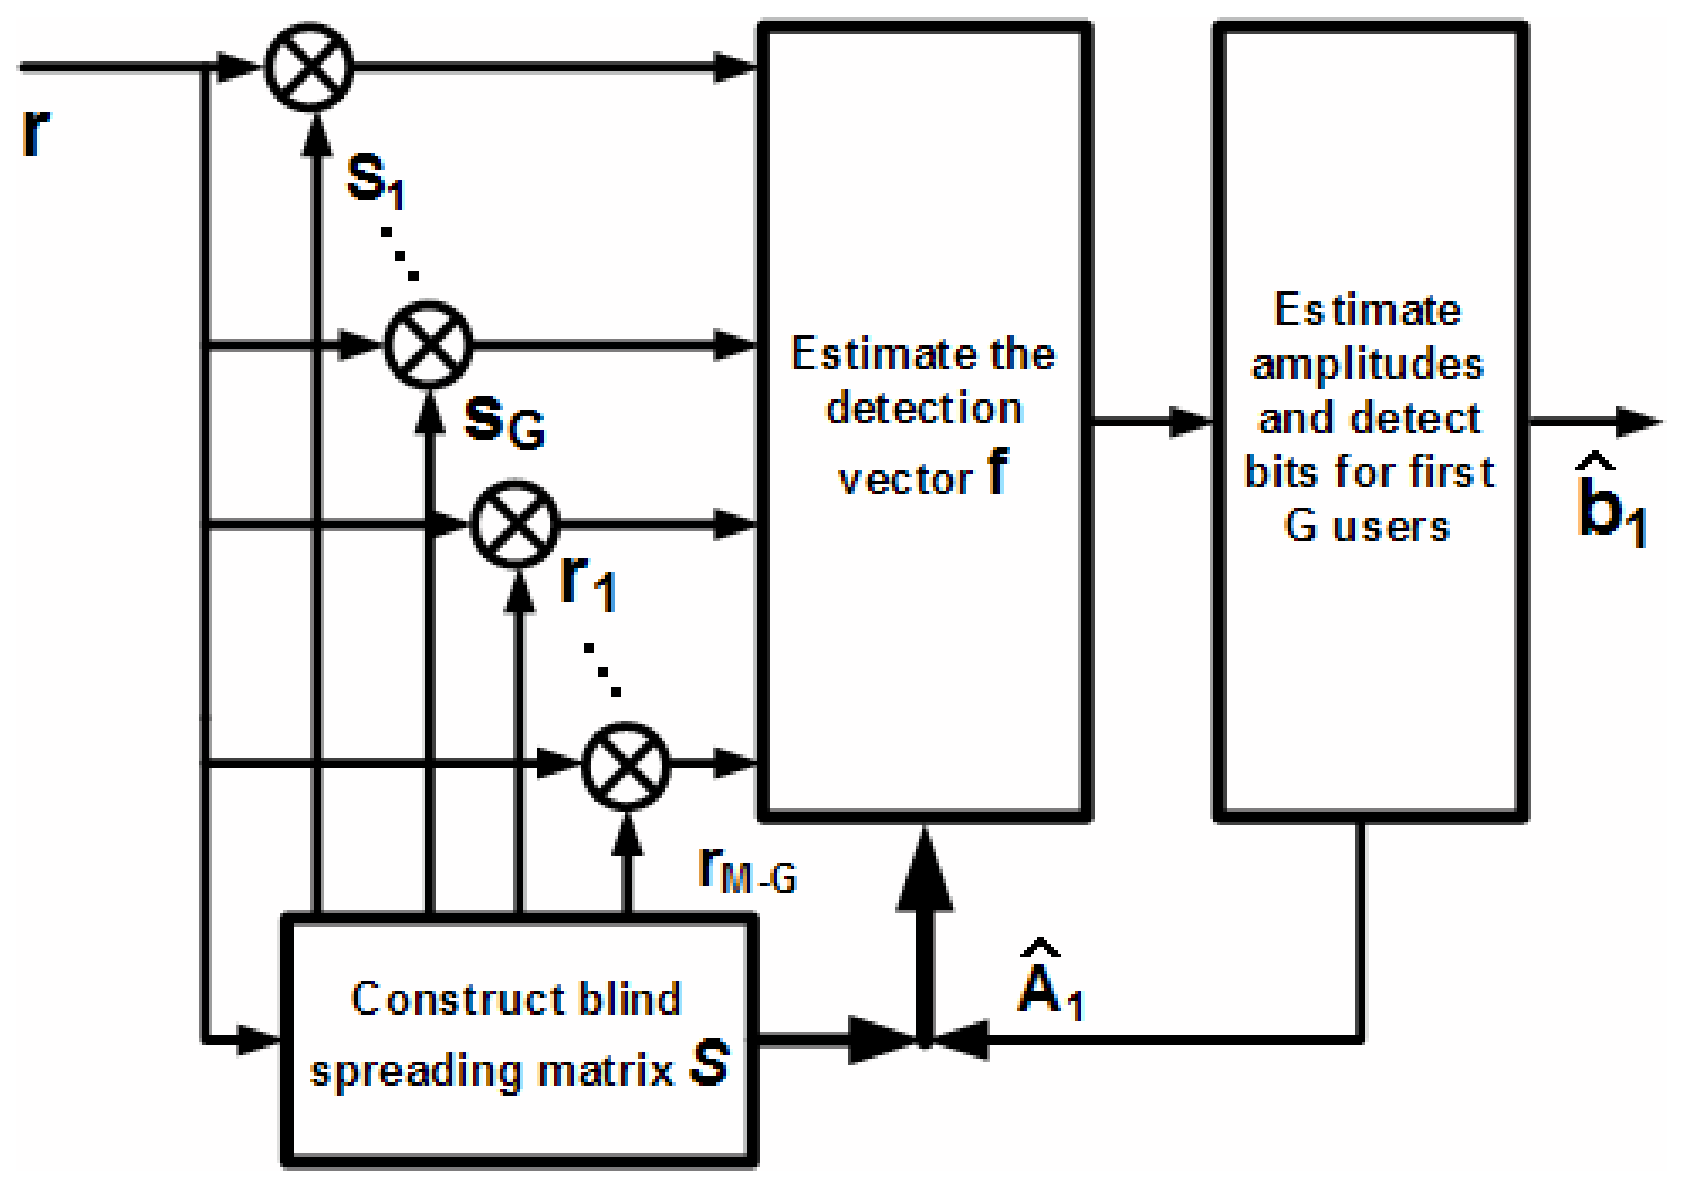
\includegraphics[width=2.5in]{BMUD_structure12.eps}
\caption{ The proposed adaptive blind multiuser detection
structure.} }\label{AMUDstruct}
\end{figure}
In Fig. 2, an adaptive structure of the presented blind multiuser
detection scheme is presented for time-variant channels. Following
the well-known Sherman-Morrison-Woodbury matrix inverse
lemma~\cite{Haykin96,Golu96}, a recursively adaptive
implementation of the proposed LS and BLU blind detector can be
expressed by
\begin{equation}\hspace{-0.0in}
\begin{array}{rcl}
\hat{\bb}_1(n)&=&\mbox{sign}\left\{\bG(n)\bcC_{\cal
S}^{+}(n)\bcS^{\rm T}(n)\br(n)\right\}
\end{array}
\end{equation}
\begin{equation}\hspace{-0.0in}
\begin{array}{l}
\bcC_{\cal S}^{+}(n)=\bcC_{\cal S}^{+}(n-1)-\frac{\bcC_{\cal
S}^{+}(n-1)\bu(n-1)\bu^{\rm T}(n-1)\bcC_{\cal
S}^{+}(n-1)}{1+\bu^{\rm T}(n-1)\bcC_{\cal S}^{+}(n-1)\bu(n-1)}
\end{array}\label{adaptiveLS}
\end{equation}
\noindent where
\begin{equation}\hspace{-0.0in}
\begin{array}{rcl}
\bcC_{\cal S}(n)&=&\bcS(n)^{\rm T}\bcS(n)
\end{array}
\end{equation}
 \noindent and $\bu(n-1)$ is designed using SVD so that
\begin{equation}\hspace{-0.00in}
\begin{array}{rcl}
\bu(n-1)\bu^{\rm T}(n-1)&=&\bcC_{\cal S}(n)-\bcC_{\cal S}(n-1)
\end{array}
\end{equation}
\section{Performance Analysis}
\subsection{AME and Near-Far Resistance}
A commonly used performance measure for a multiuser detector is
asymptotic multiuser efficiency (AME) and near-far
resistance~\cite{Verd98}. Since the proposed algorithms converges
to the conventional decorrelating detector as $\sigma^2\rightarrow
0$, their AME and near-far resistance are identical to the
decorrelating detector:
\begin{equation}
\begin{array}{rcl}
\bar{\eta}_k&=&\frac{1}{\bR_{kk}^{+}}
\end{array}.
\end{equation}
\subsection{CRLB for $\bbf$ Estimation}
The Cram\'{e}r-Rao Lower Bound (CRLB) is given by the inverse of
the Fisher information matrix (FIM). Providing the blind spreading
matrix $\bcS$ is known beforehand, we first define the parameter
vector $\mathbf{\phi} = \left[\bar{\sigma}^{2}\ \bbf^{\rm
T}\right]^{\rm T}$, where $\bar{\sigma}^{2}
=(1+\frac{M-G}{M-K})\sigma^{2}$, for computing the FIM
\begin{equation}
\begin{array}{rcl}
{\bI(\mathbf{\phi})} &=& {\rm E} \left\{ \left( \frac{\partial
\ln{\cal L}}{\partial \mathbf{\phi}} \right) \left( \frac{\partial
\ln{\cal L}}{\partial \mathbf{\phi}} \right)^{\rm H} \right\}
\label{fim}
\end{array}
\end{equation}
\noindent where $\ln{\cal L}$ is the log-likelihood function given
by
\begin{equation}
\begin{array}{rcl}
\ln{\cal
L}&=&C-L\ln\bar{\sigma}^2-\frac{1}{2\bar{\sigma}^2}\parallel\mathbf{e}\parallel_2^2
\end{array},\label{logl}
\end{equation}
\noindent $C$ is a constant and $\mathbf{e}=\br-\bcS\bbf$.
Providing $\bcS$ is known, the closed-form CRLB expression of
$\bbf$ is then given by
\begin{equation}
\begin{array}{rcl}
{\rm CRLB}(\bbf\ |\ \bcS) &
=&(1+\frac{M-G}{M-K})\sigma^{2}(\bcS^{\rm T}\bcS)^{\rm +}
\end{array}.\label{CRLB_f}
\end{equation}
\noindent It shows that the accuracy of estimating $\bbf$ may
increase with increasing $M$.
\section{Computer Simulations}
There are $K=10$ users with the group size $G=3$ and the spreading
sequences used in simulations are $64$-chip ($L=64$) random
sequences. In the computer simulations, the previous amplitude
estimation from (\ref{A_estimation}) is directly use for the next
detection without any amplitude filtering. From Subplot (a) in
Fig. 3, it is interesting to see that the performance of the
simplest LS detector has the best performance. From Subplot (b),
it is very impressive to find that the performance of blind LS
detector is very close to the conventional decorrelating detector
whatever how strong the MAI is in our simulations when $M$ is
large enough. We then check the performance of the proposed LS
blind detector against the amplitude estimation errors. From Fig.
4, we can see that the BER of the LS detector basically is
unchanged against amplitude estimation error when SNR is large
enough. From Fig. 5, we can see that the performance of the LS
detector can be better providing $M$ is larger enough. This
confirms (\ref{noise_var_new}), which shows that the variance of
$\bar{\bn}$ decrease with increasing $M$.
\begin{figure} \center{
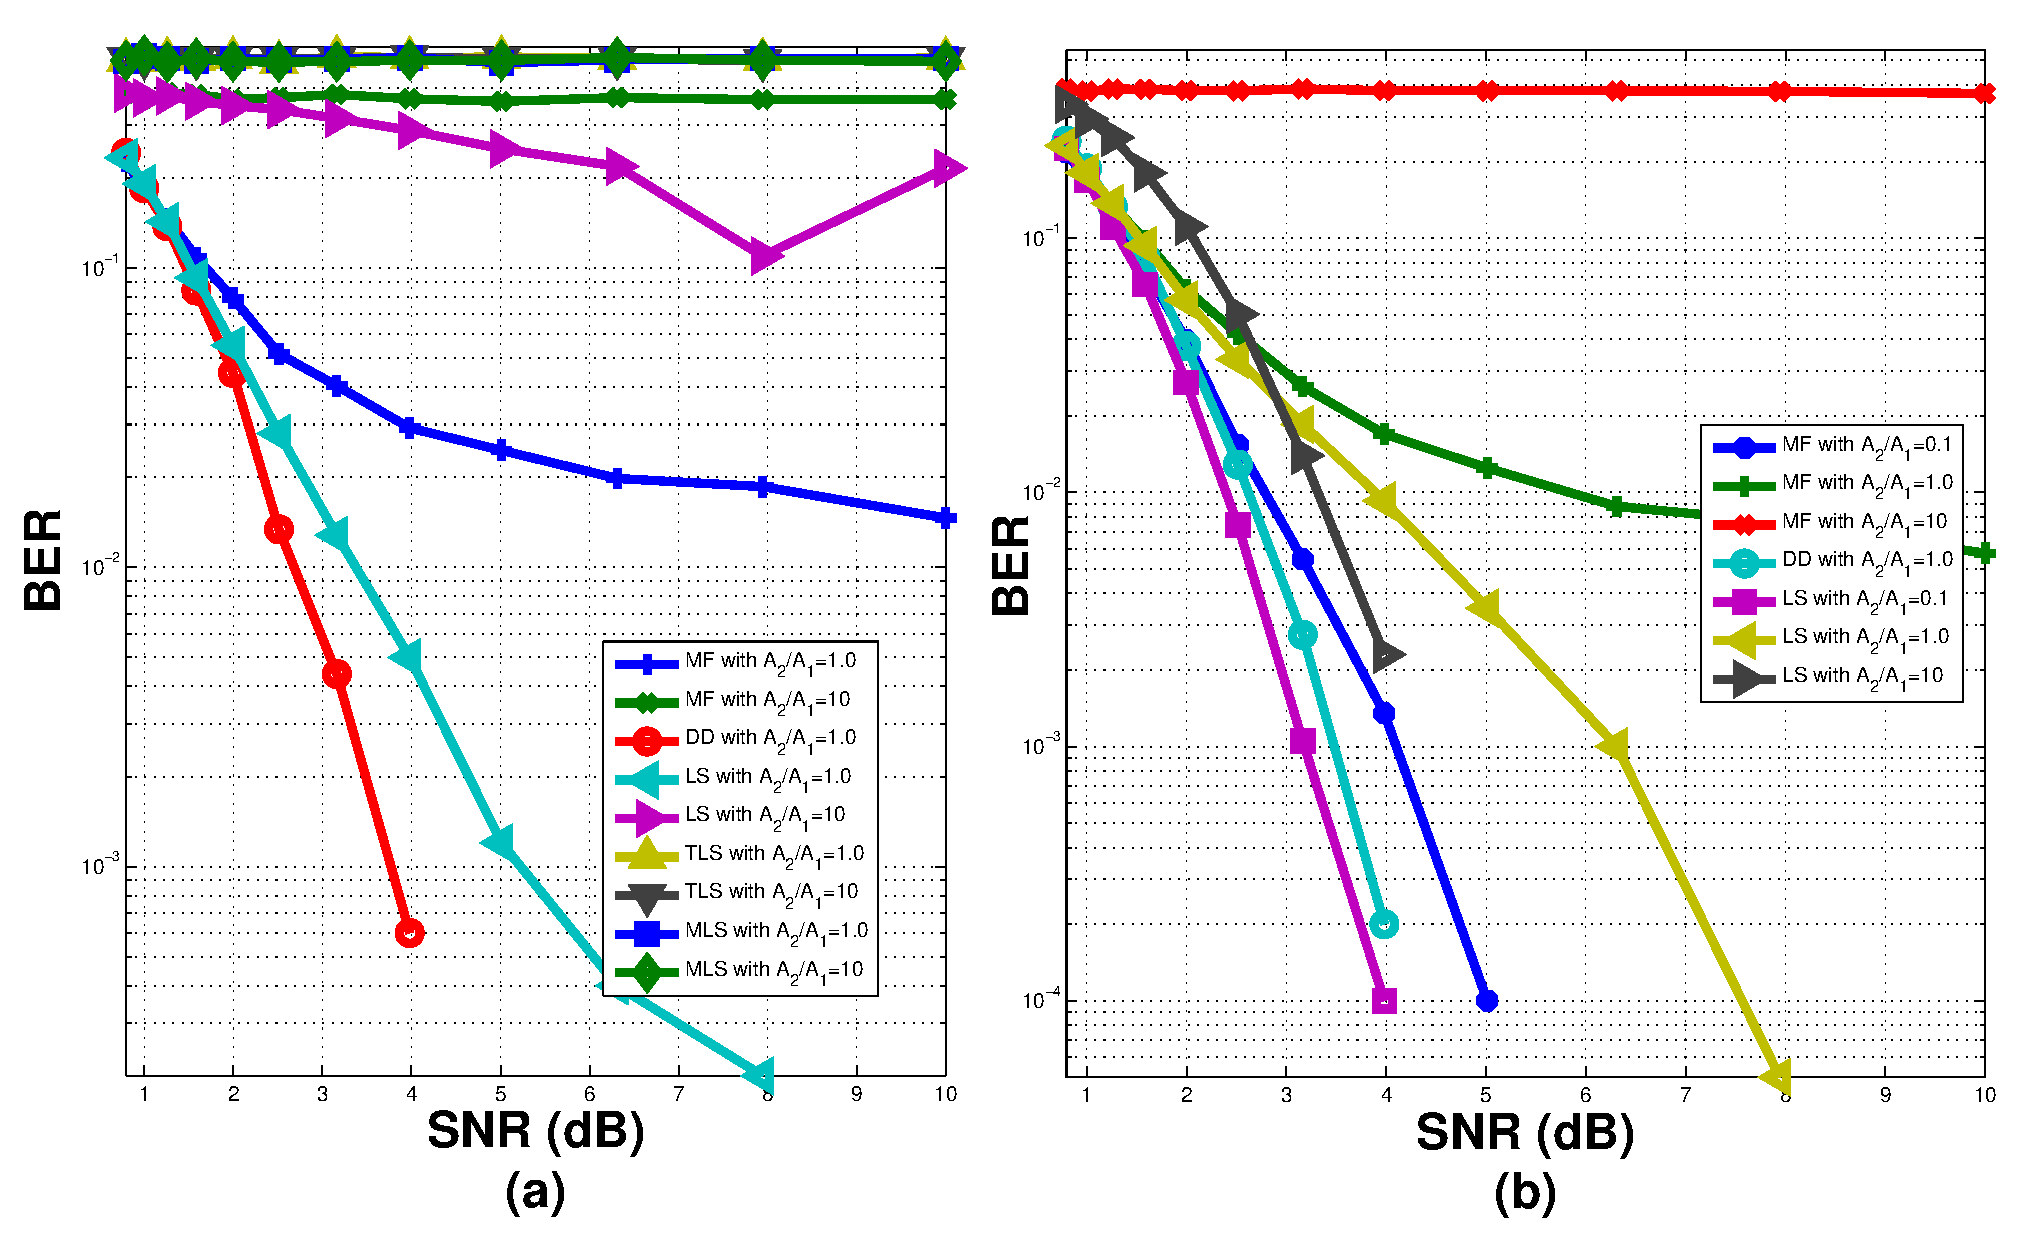
\includegraphics[width=3in]{BER_SNR_10_64.eps}
\caption{ (a) The performance of the proposed blind MUDs against
SNR, $M=12$. (b) The performance of the proposed blind LS
detector, $M=63$. } }\label{BER_SNR}
\end{figure}
\begin{figure} \center{
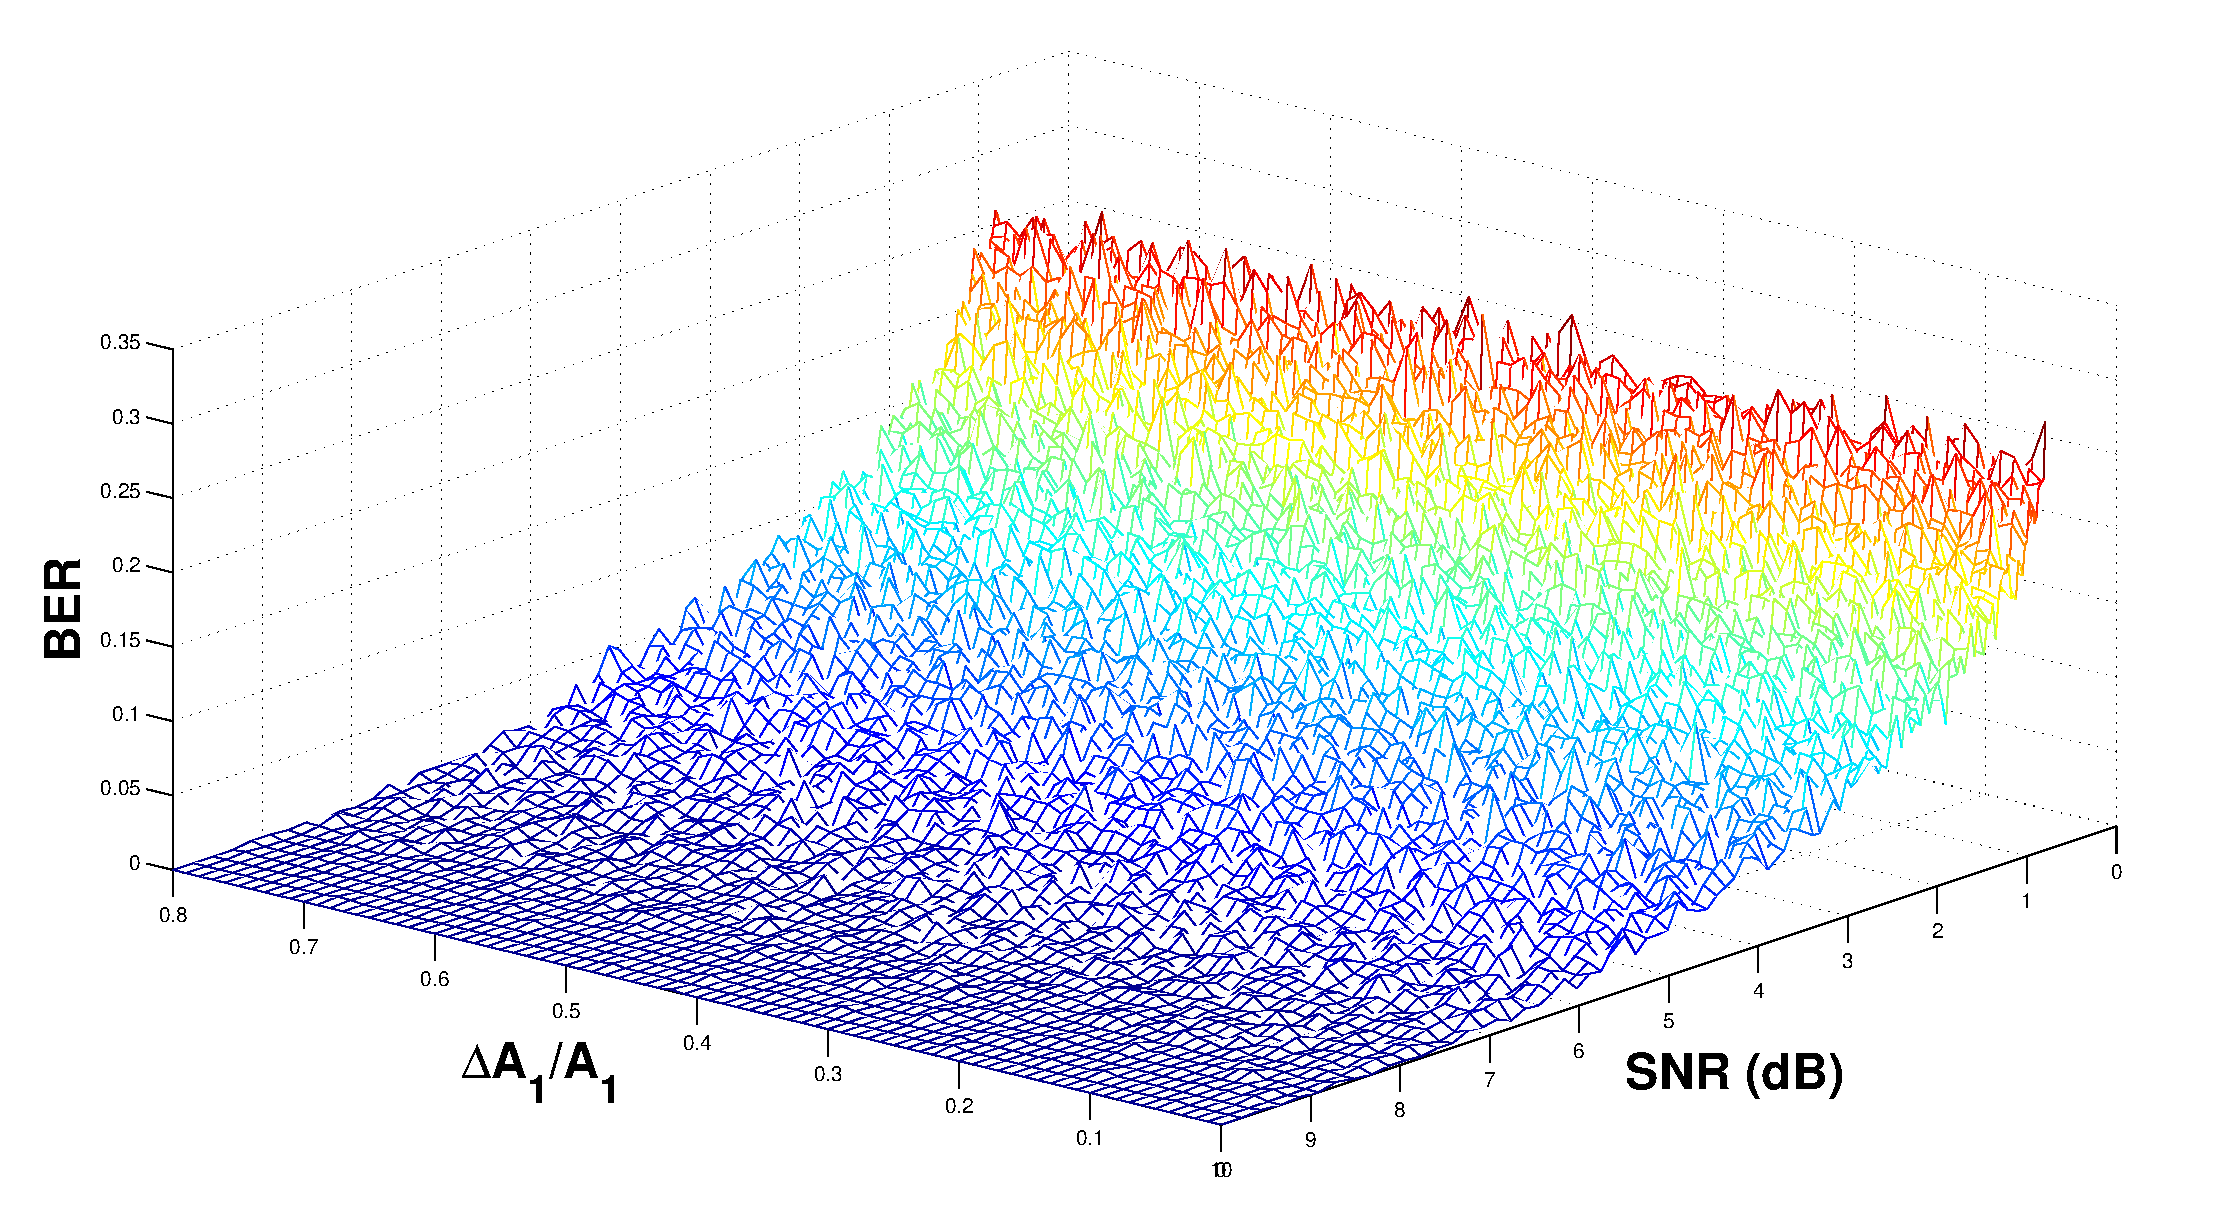
\includegraphics[width=2.5in]{BER_A_SNR_10_64_LSs.eps}
\caption{ The performance of the LS detector against amplitude
estimation error ${\Delta}{A_1}/A_1$ and SNR, $M=63$.}
}\label{BER_A_SNR}
\end{figure}
\begin{figure}
\center{
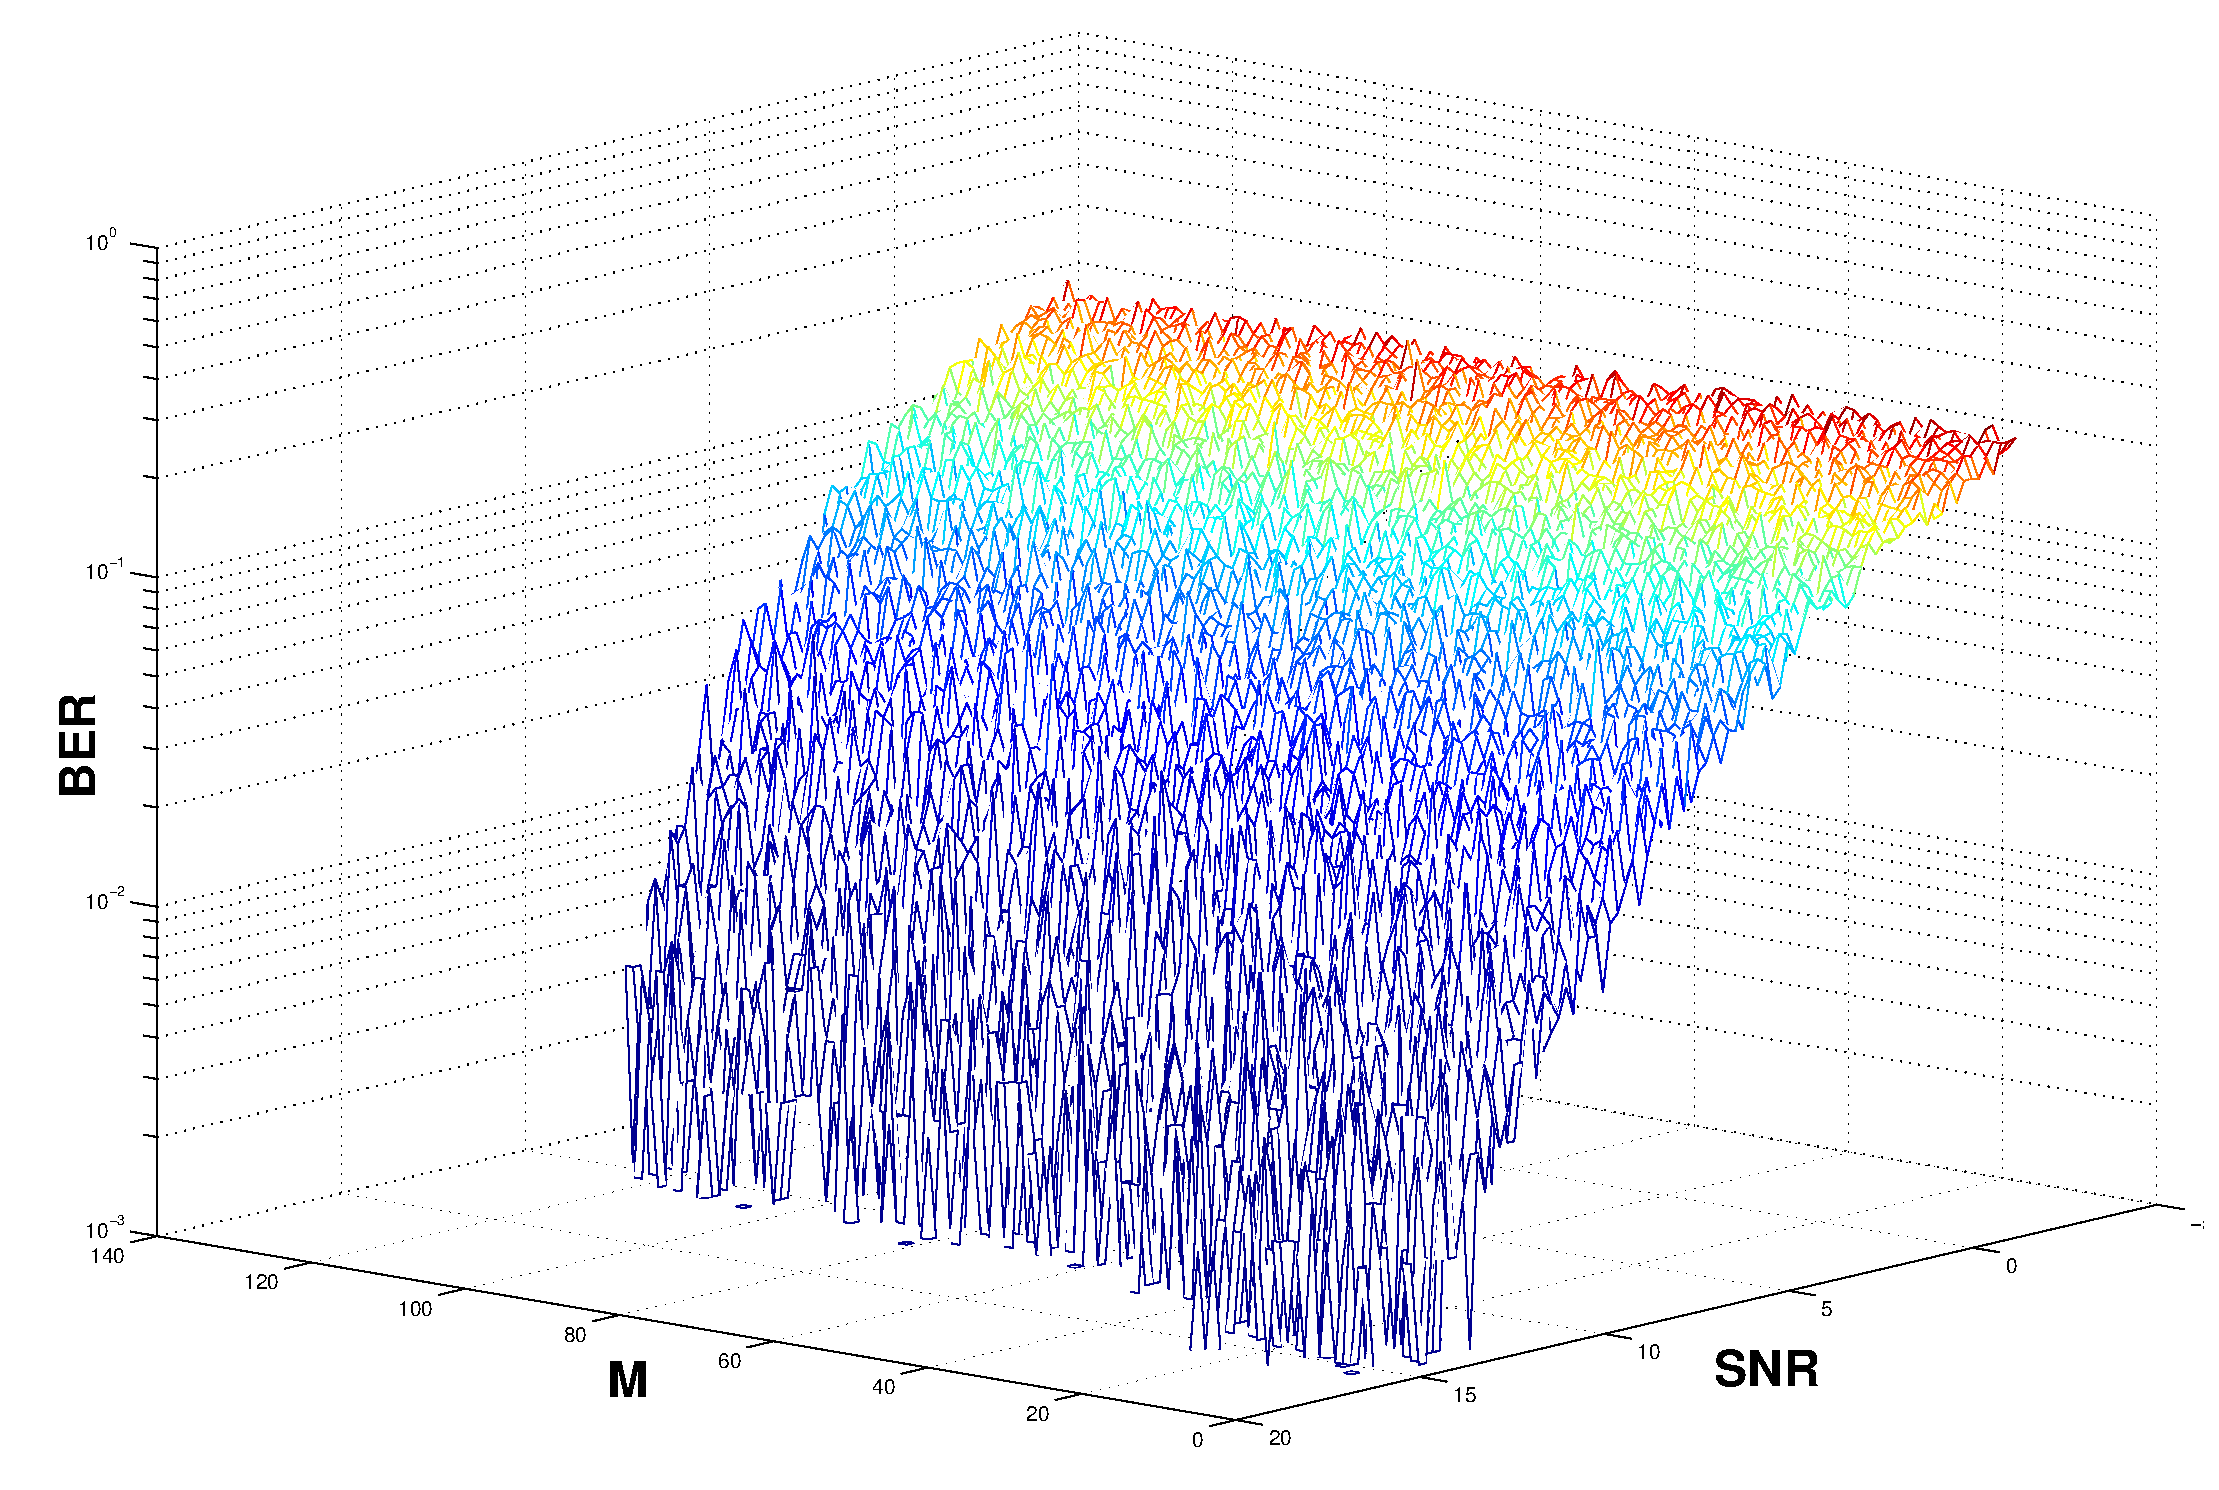
\includegraphics[width=2.5in]{BER_M_SNR_10_64_LSs.eps}
\caption{ The performance of the LS blind MUD against $M$ and
SNR.} }\label{BER_M_SNR}
\end{figure}
\section{Conclusions}
In this paper, we proposed a blind multiuser detection framework
as well as several blind detectors. The proposed blind detectors
are direct and simple without any channel or spreading sequence
estimation or subspace separation operation.
\small
\bibliographystyle{unsrt}
\bibliography{FastBDD,InterferenceCancellation}
\end{document}
